\chapter{The Simplex Method}

In Chapter~\ref{systems}, you learned how to handle systems of linear equations.
However there are many situations in which inequalities appear instead of equalities. 
In such cases we are often interested 
in an optimal solution extremizing a particular quantity of interest. 
Questions like this
are a focus of fields such as 
\href{http://en.wikipedia.org/wiki/Mathematical_optimization}{mathematical optimization}
 and 
 \href{ http://en.wikipedia.org/wiki/Operations_research}{operations research}.
For the case where the functions involved are linear,  these problems go under the
title  
\href{http://en.wikipedia.org/wiki/Linear_programming}{
{{\itshape linear programming}}\index{linear programming}}. Originally these ideas were driven by military applications,
but by now are ubiquitous in science and industry. Gigantic computers are dedicated to implementing linear programming methods such as
George Dantzig's 
\href{http://en.wikipedia.org/wiki/Simplex_algorithm}{simplex algorithm}--the topic of this chapter.

\section{Pablo's Problem}

Let us begin with an example. Consider again Pablo the nutritionist of problem~\ref{Pablo}, chapter~\ref{warmup}.
The Conundrum City school board has employed Pablo to design their school lunch program. Unfortunately for Pablo, 
their requirements are rather tricky:

\begin{example}(Pablo's problem)\\
The Conundrum City school board is heavily influenced by the local fruit grower's association. They have stipulated
that children eat at least 7 oranges and 5 apples per week. Parents and teachers have agreed that eating at least 15 pieces of fruit per
week is a good thing, but school janitors argue that too much fruit makes a terrible mess, so that children should eat no more than
25 pieces of fruit per week. 
\begin{center}
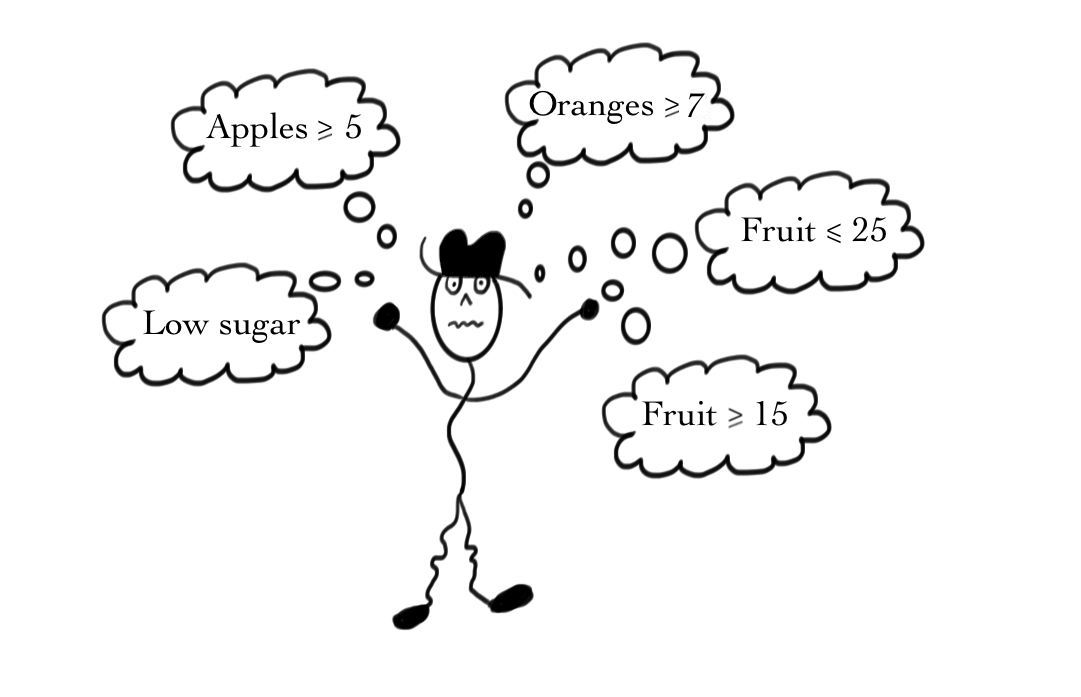
\includegraphics[scale=.3]{simplex/Pablo.jpg}
\end{center}
\noindent
Finally Pablo knows that oranges have twice as much sugar as apples
and that apples have 5 grams of sugar each. Too much sugar is unhealthy, so Pablo wants to keep the children's sugar intake as low 
as possible. How many oranges and apples should Pablo suggest that the school board put on the menu?
\end{example}

This is a rather gnarly word problem. Our first step is to restate it as mathematics, stripping away all the extraneous information:

\begin{example}(Pablo's problem restated)\\
Let $x$ be the number of apples and $y$ be the number of oranges. These must obey
\[
x\geq5\, \quad\mbox{and}\quad y\geq7\, ,
\]
to fulfill the school board's politically motivated wishes. The teacher's and parent's fruit requirement means that
\[
x+y\geq 15\, ,
\]
but to keep the canteen tidy
\[
x+y\leq 25\, .
\]
Now let 
\[s=5x+10y\, .\]
This linear function of $(x,y)$ represents the grams of sugar in $x$ apples and $y$ oranges.
The problem is asking us to minimize $s$ subject to the four linear inequalities listed above.
\end{example}

\section{Graphical Solutions}\label{graph}

Before giving a more general algorithm for handling this problem and problems like it, we note that when
the number of variables is small (preferably~2), a graphical technique can be used.

Inequalities, such as the four given in Pablo's problem, are often called {\itshape constraints}, and values of the variables that 
satisfy these constraints comprise the so-called {\itshape feasible region}. 
Since there are only two variables, this is easy to plot:

\begin{example}(Constraints and feasible region)
Pablo's constraints are
\begin{eqnarray*}
&x\geq 5&\\
&y\geq 7&\\[2mm]
&15\leq x+y\leq25\, .&
\end{eqnarray*}
Plotted in the $(x,y)$ plane, this gives:
\vspace{-5mm}
\begin{center}
\hspace{-1cm}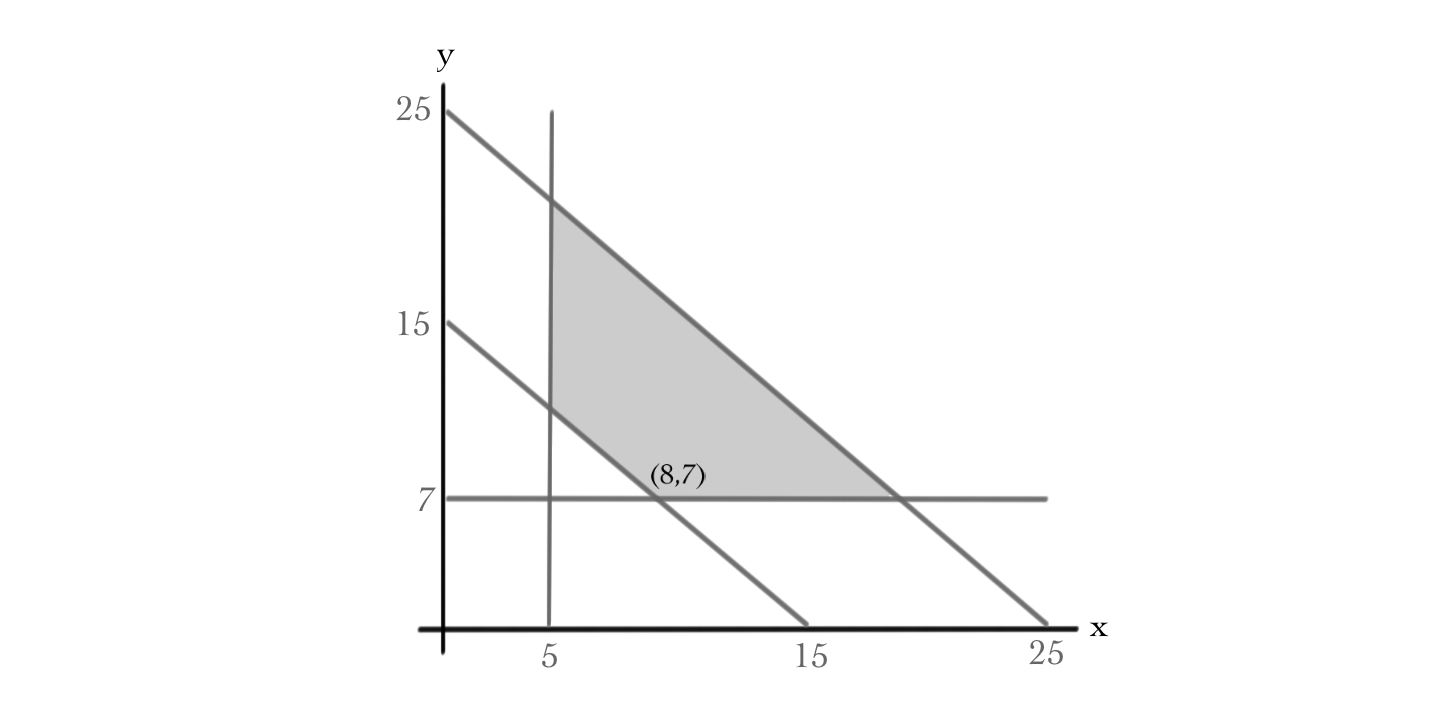
\includegraphics[scale=.32]{simplex/feasible.jpg}
\end{center}
\end{example}

You might be able to see the solution to Pablo's problem already. Oranges are very sugary, so they should be kept low, thus $y=7$.
Also, the less fruit the better, so the answer had better lie on the line $x+y=15$. Hence, the answer must be at the vertex 
$(8,7)$. Actually this is a general feature of linear programming problems, the optimal answer must lie at a vertex of the feasible region. Rather
than prove this, lets look at a plot of the linear function $s(x,y)=5x+10y$.

\begin{example}(The sugar function)\\
Plotting the sugar function requires three dimensions:
\vspace{-1.5mm}
\begin{center}
\hspace{-1cm}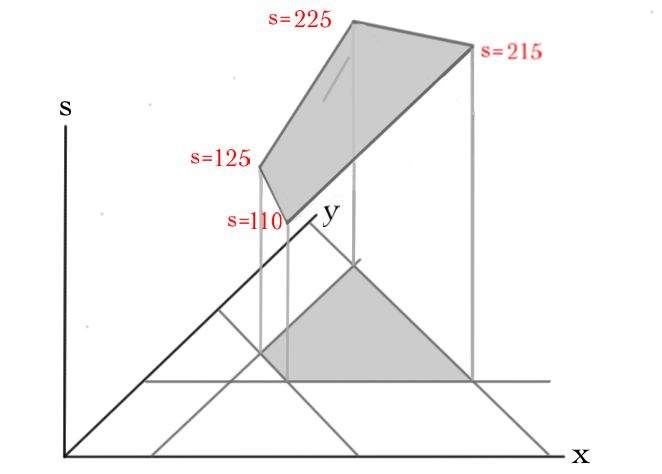
\includegraphics[scale=.38]{simplex/sugar.jpg}
\end{center}
\end{example} 

The plot of a linear function of two variables is a plane through the origin. 
Restricting the variables to the feasible region gives some lamina in 3-space.
Since the function we want to optimize is linear (and assumedly non-zero), 
if we pick a point in the middle of this lamina, we can always increase/decrease 
the function by moving out to an edge and, in turn, along that edge to a corner.
Applying this to the above picture,  we see that Pablo's best option is 110 grams of sugar a week, in the form of 
8 apples and 7 oranges.

It is worthwhile to contrast the optimization problem for a linear function with the non-linear case you may have seen in calculus courses:
\vspace{-1.5mm}
\begin{center}
\hspace{-1cm}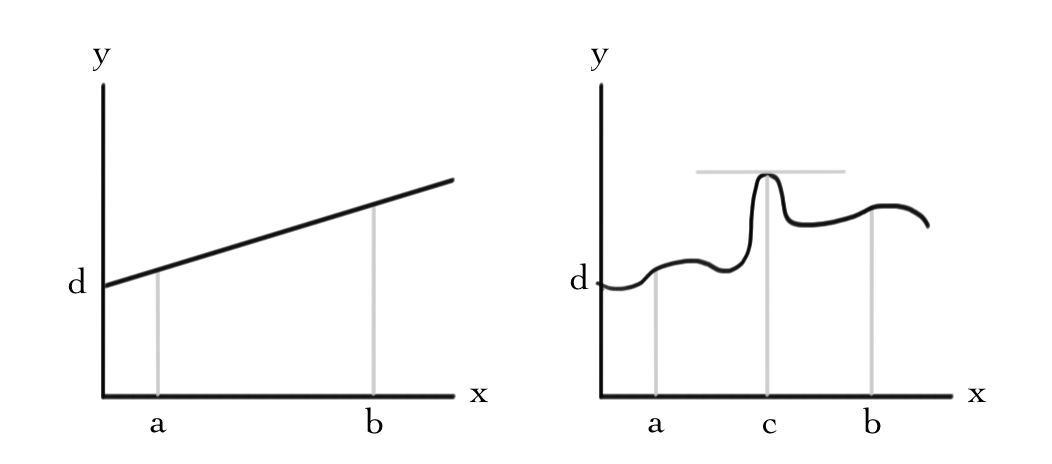
\includegraphics[scale=.33]{simplex/linvsnonlin.jpg}
\end{center}
Here we have plotted the curve $f(x)=d$ in the case where the function $f$ is linear and non-linear. 
To optimize $f$ in the interval $[a,b]$, for the linear case we just need to compute and compare the values $f(a)$ 
and $f(b)$. In contrast, for non-linear functions it is necessary to also compute the derivative $df/dx$ to study whether
there are extrema {\bf inside} the interval.

\section{Dantzig's Algorithm}\label{dantzig}

In simple situations a graphical method might suffice, but in many applications there may be thousands or even millions of variables 
and constraints. Clearly an algorithm that can be implemented on a computer is needed. The {\itshape simplex algorithm} (usually attributed to George Dantzig) provides exactly that. It begins with a standard problem:

\begin{problem}
Maximize $f(x_1,\ldots,x_n)$ where $f$ is linear, $x_i\geq 0$ ($i=1,\ldots, n$) subject~to  
\[
Mx = v\, ,\qquad x:=\ccolvec{x_1\\\vdots \\ x_n}\, ,
\]
where the $m\times n$ matrix $M$ and $m\times 1$ column vector $v$ are given.
\end{problem}
 
This is solved by arranging the information in an augmented matrix and then applying EROs.
To see how this works lets try an example.

\begin{example}\label{stdprob}
Maximize $f(x,y,z,w)=3x-3y-z+4w$ subject to constraints
\begin{equation*}
\begin{array}{rcccl}
c_1&:=&x+y+z+w&=&5\\[2mm]
c_2&:=&x+2y+3z+2w&=&6\, ,
\end{array}
\end{equation*}
where $x\geq0$, $y\geq0$, $z\geq0$ and $w\geq 0$.
\end{example}
  The key observation is this: Suppose we are trying to maximize $f(x_1,\ldots,x_n)$ subject to 
  a constraint $c(x_1,\ldots,x_n)=k$ for some constant $k$ ($c$ and $k$ would  be the entries of 
  $Mx$ and $v$, respectively, in the above). Then we can also try to maximize
  \[
 f(x_1,\ldots,x_n)+\alpha c(x_1,\ldots,x_n)\, 
  \]
  because this is only a constant shift $f\to f+\alpha k$. Choosing $\alpha$ carefully can lead to a simple form for the function we are extremizing.



\begin{example} (Setting up an augmented matrix):

Since we are interested in the optimum value of $f$, we treat it as an additional variable and add one further equation
\[
-3x+3y+z-4w+f=0\, .
\]
We arrange this equation and the two constraints in an augmented matrix
\[
\begin{array}{ccc}
\left(\begin{array}{rrrrr|r}
1&1&1&1&0&5\\[1mm]
1&2&3&2&0&6\\\hline
\!-3&3&1&\!\!-4&\ 1&\ 0
\end{array}\right)
\quad &\Leftrightarrow &% \quad 
\left\{
\begin{array}{lcl}
c_1&=&5\\[1mm]
c_2&=&6\\[1mm]
f&=&3x-3y-z+4w
\end{array}\right.
\end{array}.
\]
Keep in mind that the first four columns correspond to the positive variables $(x,y,z,w)$ and that
the last row has the information of the function $f$. The general case is depicted in figure~\ref{augD}.
\end{example}

\begin{figure}
\begin{center}
\begin{tabular}{ll}
\ \ {$\overbrace{\phantom{VERYVERYERY}}^{\mbox{\tiny variables (incl. slack and artificial)}}$}\ 
{$\overbrace{\phantom{F}}^{\mbox{\tiny objective}}$}&\\
{$
\left(
\begin{array}{c|c}
\phantom{VERYVERYERYFATS}&\phantom{S}\\
\\
\\\hline
\\
\end{array}
\right)
$} &{$\begin{array}{l} \\ \leftarrow  \mbox{constraint equations} \\[6mm] \leftarrow \mbox{objective equation}\end{array}$}\\
\hspace{4.3cm}{$\begin{array}{c}\uparrow\\ \mbox{objective value}\end{array}\!\!\!\!\!\!\!\!$}
\end{tabular}
\end{center}
\caption{Arranging the information of an optimization problem in an augmented matrix.\label{augD}}
\end{figure}



Now the system is written as an augmented matrix where the last row encodes the objective function and the other rows the constraints. Clearly 
we can perform row operations on the constraint rows since this will not change the solutions to the constraints. 
Moreover, we can add any amount of the constraint rows to the last row,
since this just amounts to adding a constant to the function we want to extremize.

\begin{example} (Performing EROs)

We scan the last row, and notice the (most negative) coefficient $-4$. Na\"ively
you might think that this is good because this multiplies the positive variable $w$
and only helps the objective function $f=4w+\cdots$. However, what this actually means
is that the variable $w$ will be positive and thus determined by the constraints. Therefore we want to remove it 
from the objective function. We can zero out this entry by performing a row operation. For that, either of the first two rows could be used. 
To decide which, we remember that  we still have to solve solve the constraints for variables that are positive. Hence we should try 
to keep the first two entries in the last column positive. Hence 
we choose the row which will add the smallest constant to $f$ when we zero out the $-4$: Look at the last column (where the values of the constraints are stored). We see that adding four times the 
first row to the last row would zero out the $-4$ entry but add $20$ to $f$, while adding two  times the second row to the last row would also zero out the $-4$ but only add $12$ to $f$. (You can follow this by watching what happens to the last entry in the last row.)
So we perform the latter row operation and obtain the following:
\[
\begin{array}{c|c}
\left(
\begin{array}{rrrrr|r}
1&1&1&1&0&5\\[1mm]
1&2&3&2&0&6\\\hline
\!-1&7&7&0&\ 1&\ 12
\end{array}\right)
\quad\quad  &\quad 
\begin{array}{rcl}
c_1&=&5\\[1mm]
c_2&=&6\\
f&=&12+x-7y-7z\, .
\end{array}
\end{array}
\]
We do not want to undo any of our good work when we perform further row operations, so now we use the second row to zero out all other entries in the fourth column. This is achieved by subtracting half the second row from the first:
\[
\begin{array}{c|c}
\left(
\begin{array}{rrrrr|r}
\frac12&0&-\frac12&0&0&2\\[1mm]
1&2&3&2&0&6\\\hline
\!-1&7&7&0&\ 1&\ 12
\end{array}\right)
\quad\quad  &\quad 
\begin{array}{rcl}
c_1-\frac12 c_2&=&2\\[1mm]
c_2&=&6\\
f&=&12+x-7y-7z\, .
\end{array}
\end{array}
\]
Precisely because we chose the second row to perform our row operations, all entries in the last column remain positive. This allows us to continue the algorithm.

We now repeat the above procedure: There is a $-1$ in the first column of the last row. We want to zero it out while adding as little to
$f$ as possible. This is achieved by adding twice the first row to the last row:
\[
\begin{array}{c|c}
\left(
\begin{array}{rrrrr|r}
\frac12&0&-\frac12&0&0&2\\[1mm]
1&2&3&2&0&6\\\hline
0&7&6&0&\ 1&\ 16
\end{array}\right)
\quad\quad  &\quad 
\begin{array}{rcl}
c_1-\frac12 c_2&=&2\\[1mm]
c_2&=&6\\
f&=&16-7y-6z\, .
\end{array}
\end{array}
\]
The Dantzig algorithm terminates if all the coefficients in the last row (save perhaps for the last entry which encodes the value of the objective) are positive.
To see why we are done, lets write out what our row operations have done in terms of the function $f$ and the constraints $(c_1,c_2)$.
First we have
\[
f=16-7y-6z
\]
with both $y$ and $z$ positive. Hence to maximize $f$ we should choose $y=0=z$. In which case we obtain our optimum value
\[
\underline{f=16\, .}
\]
Finally, we check that the constraints can be solved with $y=0=z$ and positive $(x,w)$. Indeed, they can by taking $x=4$, $w=1$.
\end{example} 

\section{Pablo Meets Dantzig} 
Oftentimes, it takes a few tricks to bring a given problem into the standard  form of example~\ref{stdprob}. In Pablo's case, this goes as follows.

\begin{example}
Pablo's variables $x$ and $y$ do not obey $x_i\geq 0$. Therefore define new variables 
\[
x_1=x-5\, , \quad x_2=y-7\, .
\]
The conditions on the fruit $15\leq x+y\leq 25$ are inequalities, 
\[
x_1+x_2\geq 3\, ,\quad x_1+x_2\leq 13\, ,
\] 
so are not of the form $Mx = v$. To achieve this we introduce two new positive variables $x_3\geq0$, $x_4\geq 4$ and write
\[
c_1:=x_1+x_2-x_3=3\, ,\quad c_2:=x_1 + x_2 + x_4=13\, .
\]
These are called {\itshape slack variables} because they take up the ``slack'' required to convert inequality to equality.
This pair of equations can now be written as $Mx=v$,
\[
\begin{pmatrix}
1 &1&\!\!-1&0\\
1&1&0&1
\end{pmatrix}
\colvec{x_1\\x_2\\x_3\\x_4}=
\colvec{3\\\!13}\, .
\]
Finally, Pablo wants to minimize sugar $s=5x+10y$, but the standard problem maximizes $f$. Thus the so-called {\itshape objective function}
$f=-s+95=-5x_1-10x_2$. (Notice that it makes no difference whether we maximize $-s$ or $-s+95$, we choose the latter since it is
a linear function of $(x_1,x_2)$.)
Now we can build an augmented matrix whose last row reflects  the objective function equation $5 x_1+10 x_2 +f=0$:
\[
\left(\begin{array}{rrrrr|r}
1&1&-1&0&0&3\\
1&1&0&1&0&13\\\hline
5&10&\ 0&0&1&0
\end{array}\right)\, .
\]
Here it seems that the simplex algorithm already terminates because the last row only has positive coefficients, so that setting $x_1=0=x_2$
would be optimal. However, this does not solve the constraints (for positive values of the slack variables $x_3$ and $x_4$).
Thus one more (very dirty) trick is needed. We add two more, positive, (so-called) {\itshape artificial variables} $x_5$ and $x_6$ to the problem
which we use to shift each constraint 
\[
c_1\to c_1-x_5\, ,\qquad c_2\to c_2-x_6\, .
\]
The idea being that for large positive~$\alpha$,  the modified objective function \[f-\alpha x_5 - \alpha x_6\]
is only maximal when the artificial variables vanish so the underlying problem is unchanged. 
Lets take $\alpha=10$ (our solution will not depend on this choice) so that our augmented matrix reads 
\begin{eqnarray*}&&
\left(\begin{array}{rrrrrrr|r}
1&1&-1&0&1&0&0&3\\
1&1&0&1&0&1&0&13\\\hline
5&10&\ 0&0&10&10&1&0
\end{array}\right)\\[2mm]
&\stackrel{\small R_3'=R_3-10 R_1-10R_2 }\sim&
\left(\begin{array}{rrrrrrr|r}
1&1&-1&0&1&0&0&3\\
1&1&0&1&0&1&0&13\\\hline
\!-15&-10&\ 10&-10&0&0&1&-160
\end{array}\right)
\, .
\end{eqnarray*}
Here we performed one row operation to zero out the coefficients of the artificial variables.
Now we are ready to run the simplex algorithm exactly as in section~\ref{dantzig}. The first row operation 
uses the~$1$ in the top of the first column to zero out the most negative entry in the last row:
\begin{eqnarray*}&&
\left(\begin{array}{rrrrrrr|r}
1&1&-1&0&1&0&0&3\\
1&1&0&1&0&1&0&13\\\hline
0&5&-5&-10&15&0&1&-115
\end{array}\right)\\[2mm]
&\stackrel{\small R_2'=R_2-R_1}\sim&
\left(\begin{array}{rrrrrrr|r}
1&1&1&0&1&0&0&3\\
0&0&1&1&-1&1&0&10\\\hline
0&5&-5&-10&15&0&1&-115
\end{array}\right)\\[2mm]
&\stackrel{\small R_3'=R_3+10R_2}\sim&
\left(\begin{array}{rrrrrrr|r}
1&1&1&0&1&0&0&3\\
0&0&1&1&-1&1&0&10\\\hline
0&5&5&0&5&10&1&-15
\end{array}\right)
\, .
\end{eqnarray*}
Now the variables $(x_2,x_3,x_5,x_6)$ have zero coefficients so must be set to zero to maximize $f$.
The optimum value is $f=-15$ so $s=-f+95=110$ exactly as before. Finally, to solve the constraints $x_1=3$
and $x_4=10$ so that $x=8$ and $y=7$ which also agrees with our previous result.
 \end{example}


Clearly, performed by hand,  the simplex algorithm was slow and complex for Pablo's problem. However, the key point is
that it is an algorithm that can be fed to a computer. For problems with many variables, this method is much faster than 
simply checking all vertices as we did in section~\ref{graph}.

\section{Review Problems}

%\section{Review Problems}






\begin{enumerate}
\item \label{det33} Let $M=\begin{pmatrix}
m^1_1 & m^1_2 & m^1_3\\
m^2_1 & m^2_2 & m^2_3\\
m^3_1 & m^3_2 & m^3_3\\
\end{pmatrix}$.  Use row operations to put $M$ into \emph{row echelon form}.  For simplicity, assume that $m_1^1\neq 0 \neq m^1_1m^2_2-m^2_1m^1_2$.

Prove that $M$ is non-singular if and only if:
\[
m^1_1m^2_2m^3_3 
- m^1_1m^2_3m^3_2 
+ m^1_2m^2_3m^3_1 
- m^1_2m^2_1m^3_3 
+ m^1_3m^2_1m^3_2
- m^1_3m^2_2m^3_1
\neq 0
\]

\phantomnewpage

\item 
\begin{enumerate}
\item What does the matrix $E^1_2=\begin{pmatrix}
0 & 1 \\
1 & 0
\end{pmatrix}$ do to $M=\begin{pmatrix}
a & b \\
d & c
\end{pmatrix}$ under left multiplication?  What about right multiplication?
\item Find elementary matrices $R^1(\lambda)$ and $R^2(\lambda)$ that respectively multiply rows $1$ and $2$ of $M$ by $\lambda$ but otherwise leave $M$ the same under left multiplication.
\item Find a matrix $S^1_2(\lambda)$ that adds a multiple $\lambda$ of row $2$ to row $1$ under left multiplication.
\end{enumerate}

\phantomnewpage

\item Let $M$ be a matrix and $S^i_jM$ the same matrix with rows \(i\) and \(j\) switched.  Explain every line of the 
\hyperlink{rowswap}{series of equations} proving that $\det M = -\det (S^i_jM)$.

\phantomnewpage

%\item \label{prob_inversion_number} This problem is a ``hands-on'' look at why \hyperlink{permutation_parity}{the property} describing the parity of permutations is true.
%
%\hypertarget{inversion_number}{The \emph{inversion number}}\index{Permutation!Inversion number} of a permutation $\sigma$ is the number of pairs $i<j$ such that $\sigma(i)>\sigma(j)$; it's the number of ``numbers that appear left of smaller numbers'' in the permutation.  For example, for the permutation $\rho = [4,2,3,1]$, the inversion number is $5$. The number $4$ comes before $2,3,$ and $1$, and $2$ and $3$ both come before $1$.
%
%Given a permutation $\sigma$, we can make a new permutation $\tau_{i,j} \sigma$ by exchanging the $i$th and $j$th entries of $\sigma$.
%
%\begin{enumerate}
%\item What is the inversion number of the permutation \(\mu=[1,2,4,3]\) that exchanges 4 and 3 and leaves everything else alone? Is it an even or an odd permutation?
%
%\item What is the inversion number of the permutation \(\rho=[4,2,3,1]\) that exchanges 1 and 4 and leaves everything else alone? Is it an even or an odd permutation?
%
%\item What is the inversion number of the permutation \(\tau_{1,3} \mu\)? Compare the parity\footnote{The \emph{parity} of an integer refers to whether the integer is even or odd. Here the parity of a permutation $\mu$ refers to the parity of its inversion number.} of \(\mu\) to the parity of \(\tau_{1,3} \mu.\)
%
%\item What is the inversion number of the permutation \(\tau_{2,4} \rho\)? Compare the parity of \(\rho\) to the parity of \(\tau_{2,4} \rho.\)
%
%\item What is the inversion number of the permutation \(\tau_{3,4} \rho\)? Compare the parity of \(\rho\) to the parity of \(\tau_{3,4} \rho.\)
%\end{enumerate}
%
%\videoscriptlink{elementary_matrices_determinant_hint.mp4}{Problem~\ref{prob_inversion_number} hints}{scripts_elementary_matrices_determinants_hint}

\phantomnewpage

%\item \label{problem_permutation} (Extra credit) Here we will examine a (very) small set of the general properties about permutations and their applications. In particular, we will show that one way to compute the sign of a permutation is by finding the \hyperlink{inversion_number}{inversion number} $N$ of $\sigma$ and we have
%\[
%\sgn(\sigma) = (-1)^N.
%\]
%
%For this problem, let $\mu = [1,2,4,3]$.
%
%\begin{enumerate}
%\item Show that every permutation $\sigma$ can be sorted by only taking simple (adjacent) transpositions\index{Permutation!Simple transposition} $s_i$ where $s_i$ interchanges the numbers in position $i$ and $i+1$ of a permutation $\sigma$ (in our other notation $s_i = \tau_{i,i+1}$). For example $s_2 \mu = [1, 4, 2, 3]$, and to sort $\mu$ we have $s_3 \mu = [1, 2, 3, 4]$.
%
%\item \label{prob_part_relations} We can compose simple transpositions together to represent a permutation (note that the sequence of compositions is not unique), and these are associative, we have an identity (the trivial permutation where the list is in order or we do nothing on our list), and we have an inverse since it is clear that $s_i s_i \sigma = \sigma$. Thus permutations of $[n]$ under composition are an example of a \hyperref[groups]{group}. However note that not all simple transpositions commute with each other since
%\begin{align*}
%s_1 s_2 [1, 2, 3] & = s_1 [1, 3, 2] = [3, 1, 2]
%\\ s_2 s_1 [1, 2, 3] & = s_2 [2, 1, 3] = [2, 3, 1]
%\end{align*}
%(you will prove here when simple transpositions commute). When we consider our initial permutation to be the trivial permutation $e = [1, 2, \dotsc, n]$, we do not write it; for example $s_i \equiv s_i e$ and $\mu = s_3 \equiv s_3 e$. This is analogous to not writing 1 when multiplying. Show that $s_i s_i = e$ (in shorthand $s_i^2 = e$), $s_{i+1} s_i s_{i+1} = s_i s_{i+1} s_i$ for all $i$, and $s_i$ and $s_j$ commute for all $|i - j| \geq 2$.
%
%\item Show that every way of expressing $\sigma$ can be obtained from using the relations proved in part~\ref{prob_part_relations}. In other words, show that for any expression $w$ of simple transpositions representing the trivial permutation $e$, using the proved relations.
%
%\emph{Hint: Use induction on $n$. For the induction step, follow the path of the $(n+1)$-th strand by looking at $s_n s_{n-1} \cdots s_k s_{k\pm1} \cdots s_n$ and argue why you can write this as a subexpression for any expression of $e$. Consider using diagrams of these paths to help.}
%
%\item The simple transpositions \hyperlink{action}{acts on} an $n$-dimensional vector space $V$ by $s_i v = E^i_{i+1} v$ (where $E^i_j$ is \hyperlink{elem_matrix_row_swap}{an elementary matrix}) for all vectors $v \in V$. Therefore we can just represent a permutation $\sigma$ as the matrix $M_{\sigma}$\footnote{Often people will just use $\sigma$ for the matrix when the context is clear.}, and we have $\det(M_{s_i}) = \det(E^i_{i+1}) = -1$. Thus prove that $\det(M_{\sigma}) = (-1)^N$ where $N$ is a number of simple transpositions needed to represent $\sigma$ as a permutation. You can assume that $M_{s_i s_j} = M_{s_i} M_{s_j}$ (it is not hard to prove) and that $\det(A B) = \det(A) \det(B)$ \hyperref[detmultiplicative]{from Chapter~\ref*{elementarydeterminantsII}}.
%
%\emph{Hint: You to make sure $\det(M_{\sigma})$ is well-defined since there are infinite ways to represent $\sigma$ as simple transpositions.}
%
%\item Show that $s_{i+1} s_i s_{i+1} = \tau_{i, i+2}$, and so give one way of writing $\tau_{i, j}$ in terms of simple transpositions? Is $\tau_{i,j}$ an even or an odd permutation? What is $\det(M_{\tau_{i,j}})$? What is the inversion number of $\tau_{i,j}$?
%
%\item The minimal number of simple transpositions needed to express $\sigma$ is called the \emph{length}\index{Permutation!Length} of $\sigma$; for example the length of $\mu$ is 1 since $\mu = s_3$. Show that the length of $\sigma$ is equal to the inversion number of $\sigma$.
%
%\emph{Hint: Find an procedure which gives you a new permutation $\sigma^{\prime}$ where $\sigma = s_i \sigma^{\prime}$ for some $i$ and the inversion number for $\sigma^{\prime}$ is 1 less than the inversion number for $\sigma$.}
%
%\item Show that $(-1)^N = \sgn(\sigma) = \det(M_{\sigma})$, where $\sigma$ is a permutation with $N$ inversions. Note that this immediately implies that $\sgn(\sigma \rho) = \sgn(\sigma) \sgn(\rho)$ for any permutations $\sigma$ and $\rho$.
%\end{enumerate}

\item Let $M'$ be the matrix obtained from $M$ by swapping two columns $i$ and $j$. Show that $\det M'=-\det M $.

\item The scalar triple product of three vectors $u,v,w$ from $\Re^3$ is $u\cdot(v\times w)$. Show that this product is the same as the determinant of the matrix whose columns are $u,v,w$ (in that order). What happens to the scalar triple product when the factors are permuted? 

\item Show that if $M$ is a $3\times 3$ matrix whose third row is a sum of multiples of the other rows ($R_3=aR_2+bR_1$) then $\det M=0$. Show that the same is true if one of the columns is a sum of multiples of the others. 

\end{enumerate}

\phantomnewpage

